\documentclass{article}

% Language setting
% Replace `english' with e.g. `spanish' to change the document language
\usepackage[english]{babel}
\usepackage{fontawesome5}
% Set page size and margins
% Replace `letterpaper' with `a4paper' for UK/EU standard size
\usepackage[letterpaper,top=2cm,bottom=2cm,left=3cm,right=3cm,marginparwidth=1.75cm]{geometry}

% Useful packages
\usepackage{amsmath}
\usepackage{graphicx}
\usepackage[colorlinks=true, allcolors=blue]{hyperref}

\title{Problem Set 5}
\author{JaeSeok Oh}

\begin{document}
	\maketitle
	
	\begin{large}
		\section*{Q3.}
		
		\begin{itemize}
			\item I scraped a data set from \textit{StockX}\footnote{url{https://stockx.com/air-jordan-1-low-fragment-design-x-travis-scott}} website which is a popular platform for selling and buying sneakers, electronics, and clothings. The `url' I noted in the foot of this page is the exact page for the sneakers I want to look at.
			\begin{figure}[h]
				\caption{Jordan 1 Retro Low OG SP Fragment $ \times $ Travis Scott}
				\centering
				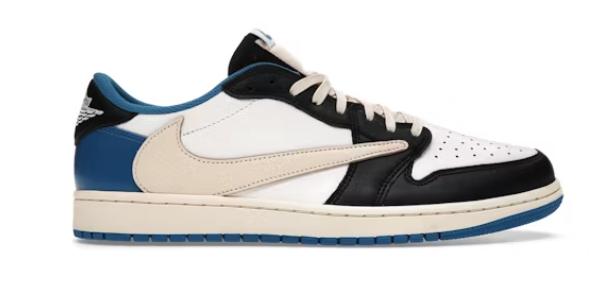
\includegraphics[width = 100mm]{TS.png}
			\end{figure}
			\item The data set consist of exact date and time when one transaction between buyer and seller was made, and the price of the transaction. Since I scraped the data set only for US M 10.5 size, the size is the same across all transaction in the data set.
			\item The website has recorded every transaction in the platform so that we can chase the price pattern. The transaction is resulted from the dynamic interaction between sellers and buyers; therefore, I would expect a decrease in prices. The most important part of this secondary market of sneakers is `popularity' among people, which means as time goes, the willingness to pay is likely to decrease.
			\item I can also scrape the number of bids and asks so that I can combine that data with this data to see how the number of bids and asks has impacts on the price for the next transaction. Moreover, Moreover, I can track price patterns not only in the short term but also in the long term, such as one year after release.
			\item To do this, I learned Python codes from  \faYoutube Youtube `Tech With Tim' tutorial 1 through 4.
		\end{itemize}
		
		\section*{Q4.}
		\begin{itemize}
			\item I scape the data sets from FRED(Rederal Reserve Bank of St Louis). First data(\textcolor{red}{the number of retail stores}) shows the changes of the number of stores over time. Second data(\textcolor{blue}{expenditures on footwear}) shows the changes of the value spending on footwear. It is clear that the change around COVID19 period was much larger for the number of stores than the expenditure spending.
				\begin{figure}[h]
				\caption{Compare Number of Retail Stores(log) to Customer Expenditure(log)}
				\centering
				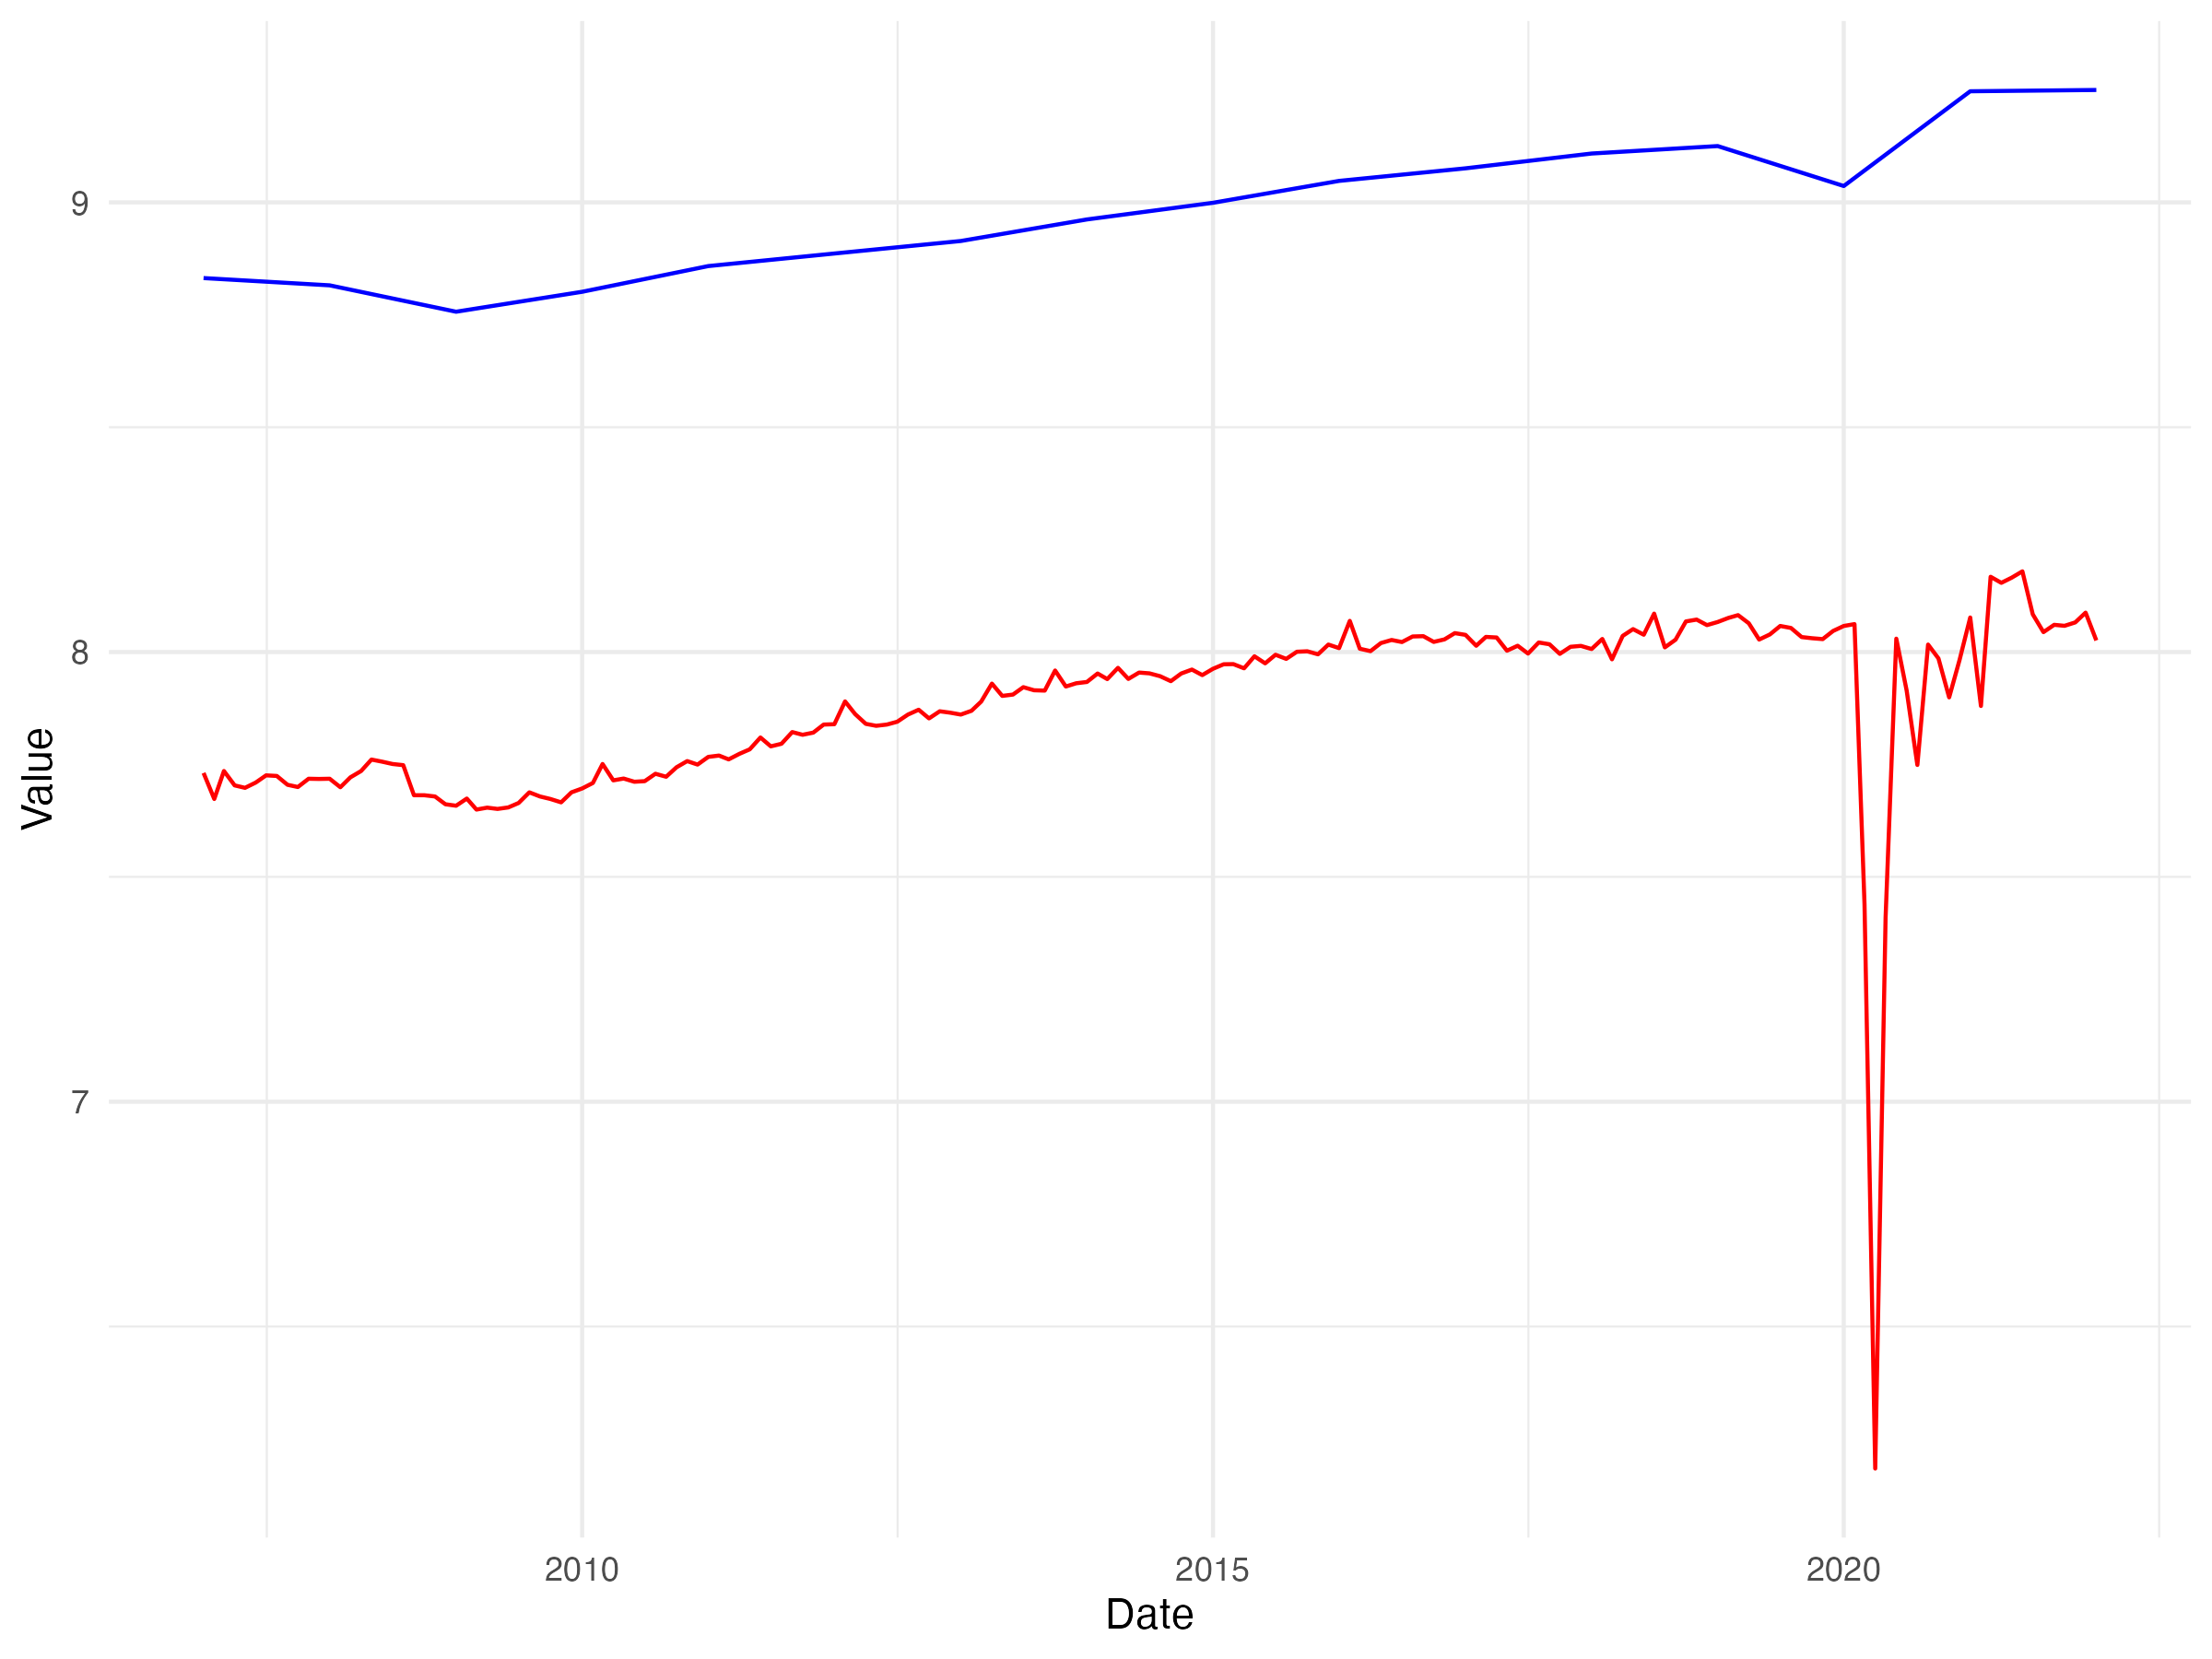
\includegraphics[width = 100mm]{plot.png}
				\label{fig2}
			\end{figure}
			\item This is interesting because many platforms have boomed after COVID19. When I talked with an undergraduate student, the student said that during COVID19, many influencers shown them through `Tiktok', `Instragram', or the other SNS, which leads sneakers to get `hyped'. Surprisingly, the prices of sneakers in the online platform(\textit{e.g.} StockX) was increasing fastly during the pandemic. According to the \textcolor{blue}{Figure} \ref{fig2}, even the number of stores decreased dractically, the expenditure on shoe seems not in a serious decrease. Therefore, it might be reasonable to look at the relationship between the online sneakers platform and SNS.
			\item I did use `httr' and `jsonlite'.
		\end{itemize}
		
		
		
		
		
	\end{large}
\end{document}